% =============================================================================
% Graphical overview for the GitHub README.  Standalone TikZ.
% Every number here is taken from the corrected manuscript (Table 1, Fig. 2C,
% Results).  Layout is on an explicit cm grid; every text node has a declared
% width smaller than the box it sits in.
% =============================================================================
\documentclass[border=0pt]{standalone}
\usepackage[T1]{fontenc}
\usepackage[scaled=0.95]{helvet}
\renewcommand{\familydefault}{\sfdefault}
\usepackage{tikz}
\usetikzlibrary{arrows.meta,shapes.geometric}
\hyphenpenalty=10000 \exhyphenpenalty=10000

\definecolor{navy}{RGB}{0,47,87}
\definecolor{steel}{RGB}{144,160,188}
\definecolor{sage}{RGB}{129,178,154}
\definecolor{rose}{RGB}{186,122,129}
\definecolor{sand}{RGB}{182,144,101}
\definecolor{apri}{RGB}{226,146,60}
\definecolor{ink}{RGB}{38,44,54}
\definecolor{mute}{RGB}{108,116,128}
\definecolor{paper}{RGB}{255,255,255}
\definecolor{panel}{RGB}{246,247,249}
\definecolor{rule}{RGB}{222,226,232}

\tikzset{
  colhead/.style={font=\bfseries\large, text=navy, anchor=west},
  colnum/.style={circle, fill=navy, text=white, font=\bfseries\small,
                 inner sep=0pt, minimum size=6mm},
  lbl/.style={font=\small, text=ink, anchor=west, align=left, text width=2.9cm, inner sep=0pt},
  val/.style={font=\small\bfseries, text=ink, anchor=west, inner sep=0pt},
  pill/.style={rounded corners=2.6mm, minimum width=1.05cm, minimum height=0.52cm,
               font=\small\bfseries, text=white, inner sep=0pt},
  card/.style={draw=rule, fill=paper, rounded corners=3pt, line width=0.6pt},
  big/.style={font=\bfseries\Large, text=navy, anchor=west, inner sep=0pt},
  ctext/.style={font=\small, text=ink, anchor=west, align=left, text width=4.0cm, inner sep=0pt},
  flow/.style={-{Stealth[length=3mm,width=2.4mm]}, line width=1.1pt, draw=navy!55},
}

\begin{document}
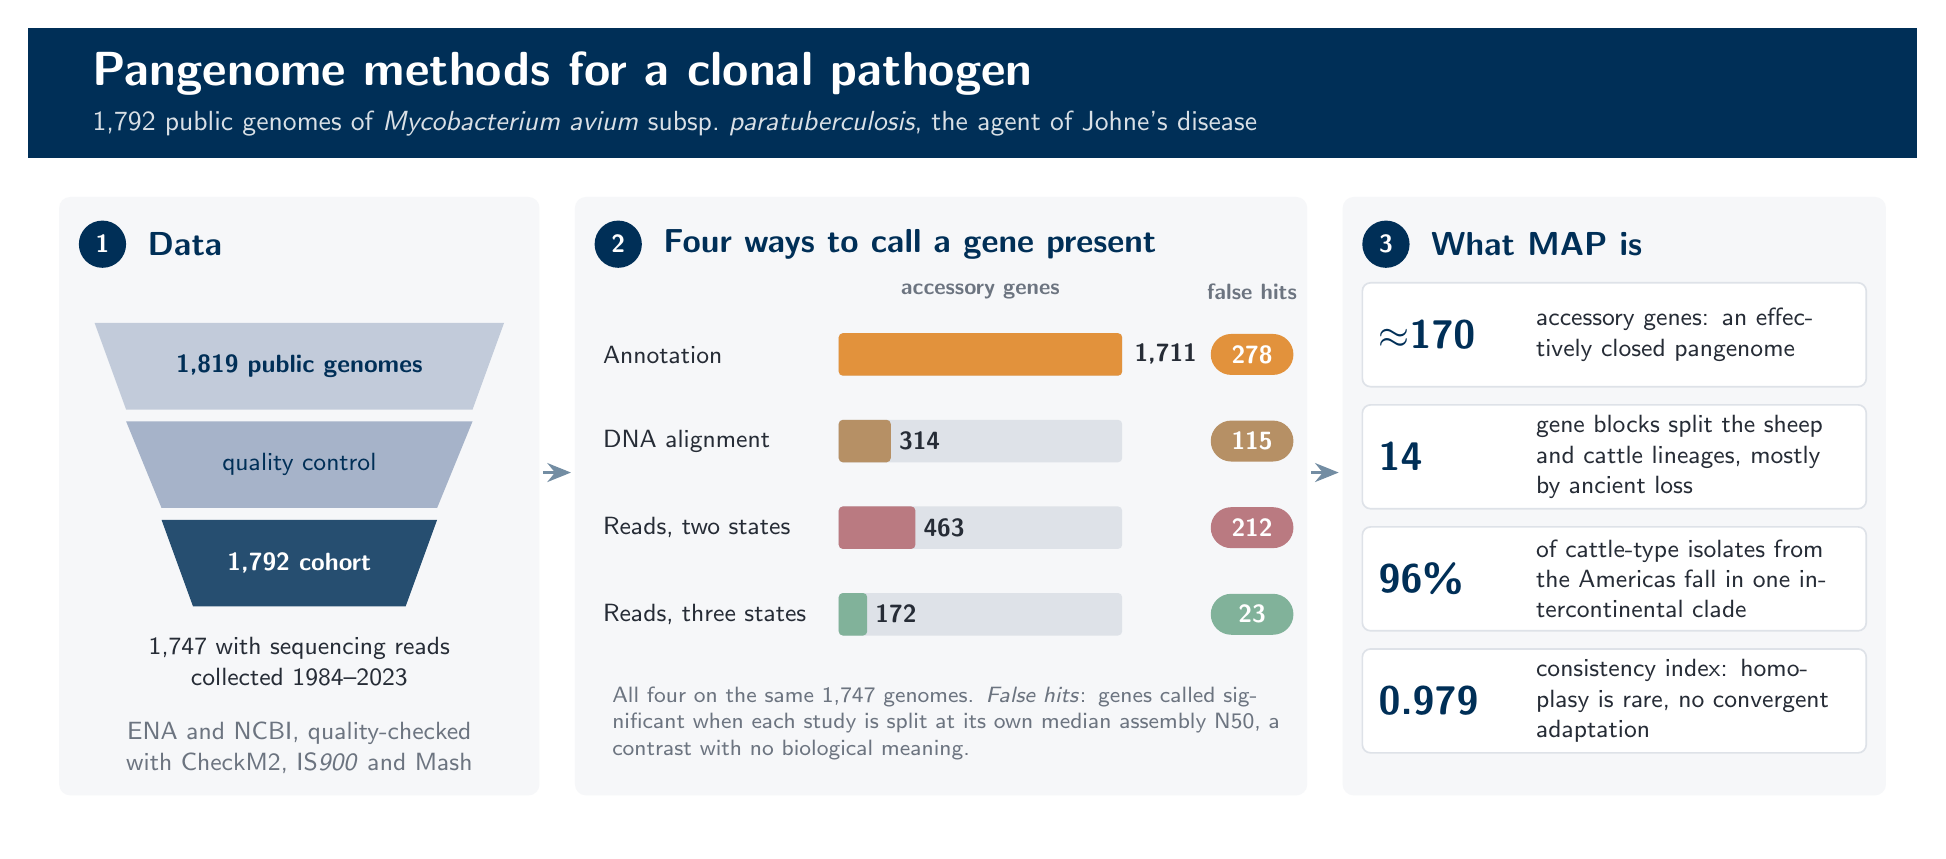
\begin{tikzpicture}

% ---------- canvas -----------------------------------------------------------
\fill[paper] (0,0) rectangle (24,10.2);
\fill[navy, rounded corners=0pt] (0,8.55) rectangle (24,10.2);
\node[anchor=west, font=\bfseries\LARGE, text=white] at (0.7,9.62)
  {Pangenome methods for a clonal pathogen};
\node[anchor=west, font=\normalsize, text=white!85!navy] at (0.7,8.98)
  {1,792 public genomes of \textit{Mycobacterium avium} subsp.\ \textit{paratuberculosis}, the agent of Johne's disease};

% column panels
\fill[panel, rounded corners=4pt] (0.40,0.45) rectangle (6.50,8.05);
\fill[panel, rounded corners=4pt] (6.95,0.45) rectangle (16.25,8.05);
\fill[panel, rounded corners=4pt] (16.70,0.45) rectangle (23.60,8.05);

% ---------- column 1: data -------------------------------------------------
\node[colnum] at (0.95,7.45) {1};
\node[colhead] at (1.40,7.45) {Data};

\fill[steel!55]  (0.85,6.45) -- (6.05,6.45) -- (5.65,5.35) -- (1.25,5.35) -- cycle;
\fill[steel!80]  (1.25,5.20) -- (5.65,5.20) -- (5.20,4.10) -- (1.70,4.10) -- cycle;
\fill[navy!85]   (1.70,3.95) -- (5.20,3.95) -- (4.80,2.85) -- (2.10,2.85) -- cycle;
\node[font=\small\bfseries, text=navy, align=center] at (3.45,5.90) {1,819 public genomes};
\node[font=\small, text=navy, align=center] at (3.45,4.65) {quality control};
\node[font=\small\bfseries, text=white, align=center] at (3.45,3.40) {1,792 cohort};

\node[font=\small, text=ink, align=center, text width=5.4cm] at (3.45,2.15)
  {1,747 with sequencing reads\\collected 1984--2023};
\node[font=\small, text=mute, align=center, text width=5.4cm] at (3.45,1.05)
  {ENA and NCBI, quality-checked\\with CheckM2, IS\textit{900} and Mash};

% ---------- column 2: four presence calls ----------------------------------
\node[colnum] at (7.50,7.45) {2};
\node[colhead] at (7.95,7.45) {Four ways to call a gene present};

\node[font=\footnotesize\bfseries, text=mute] at (12.10,6.85) {accessory genes};
\node[font=\footnotesize\bfseries, text=mute] at (15.55,6.85) {false hits};

% bars: 3.6 cm = 1,711 genes
\foreach \y/\name/\len/\col in {
    6.05/{Annotation}/3.600/apri,
    4.95/{DNA alignment}/0.661/sand,
    3.85/{Reads, two states}/0.974/rose,
    2.75/{Reads, three states}/0.362/sage} {
  \node[lbl] at (7.30,\y) {\name};
  \fill[rule, rounded corners=1.5pt] (10.30,\y-0.27) rectangle (13.90,\y+0.27);
  \fill[\col, rounded corners=1.5pt] (10.30,\y-0.27) rectangle (10.30+\len,\y+0.27);
}
\node[val] at (14.05,6.05) {1,711};
\node[val] at (11.06,4.95) {314};
\node[val] at (11.37,3.85) {463};
\node[val] at (10.76,2.75) {172};

\node[pill, fill=apri] at (15.55,6.05) {278};
\node[pill, fill=sand] at (15.55,4.95) {115};
\node[pill, fill=rose] at (15.55,3.85) {212};
\node[pill, fill=sage] at (15.55,2.75) {23};

\node[font=\footnotesize, text=mute, anchor=north west, align=left, text width=8.6cm]
  at (7.30,1.95)
  {All four on the same 1,747 genomes. \textit{False hits}: genes called
   significant when each study is split at its own median assembly N50,
   a contrast with no biological meaning.};

% ---------- column 3: findings ---------------------------------------------
\node[colnum] at (17.25,7.45) {3};
\node[colhead] at (17.70,7.45) {What MAP is};

\foreach \y/\big/\txt in {
    6.30/{$\approx$170}/{accessory genes: an effectively closed pangenome},
    4.75/{14}/{gene blocks split the sheep and cattle lineages, mostly by ancient loss},
    3.20/{96\%}/{of cattle-type isolates from the Americas fall in one intercontinental clade},
    1.65/{0.979}/{consistency index: homoplasy is rare, no convergent adaptation}} {
  \draw[card] (16.95,\y-0.66) rectangle (23.35,\y+0.66);
  \node[big] at (17.15,\y) {\big};
  \node[ctext] at (19.15,\y) {\txt};
}

% ---------- flow arrows between columns ------------------------------------
\draw[flow] (6.55,4.55) -- (6.90,4.55);
\draw[flow] (16.30,4.55) -- (16.65,4.55);

\end{tikzpicture}
\end{document}
